%
% This is the LaTeX template file for lecture notes for EE 382C/EE 361C.
%
% To familiarize yourself with this template, the body contains
% some examples of its use.  Look them over.  Then you can
% run LaTeX on this file.  After you have LaTeXed this file then
% you can look over the result either by printing it out with
% dvips or using xdvi.
%
% This template is based on the template for Prof. Sinclair's CS 270.

\documentclass[twoside]{article}
\usepackage{graphicx}
\setlength{\oddsidemargin}{0.25 in}
\setlength{\evensidemargin}{-0.25 in}
\setlength{\topmargin}{-0.6 in}
\setlength{\textwidth}{6.5 in}
\setlength{\textheight}{8.5 in}
\setlength{\headsep}{0.75 in}
\setlength{\parindent}{0.25 in}
\setlength{\parskip}{0.1 in}

\usepackage{caption} 
\usepackage{algorithm}
\usepackage{listings}
\newcommand{\forceindent}{\leavevmode{\parindent=2em\indent}}
\newcounter{magicrownumbers}
\newcommand\rownumber{\stepcounter{magicrownumbers}\arabic{magicrownumbers}}
\usepackage[colorlinks]{hyperref}

%
% The following commands set up the lecnum (lecture number)
% counter and make various numbering schemes work relative
% to the lecture number.
%
\newcounter{lecnum}
\renewcommand{\thepage}{\thelecnum-\arabic{page}}
\renewcommand{\thesection}{\thelecnum.\arabic{section}}
\renewcommand{\theequation}{\thelecnum.\arabic{equation}}
\renewcommand{\thefigure}{\thelecnum.\arabic{figure}}
\renewcommand{\thetable}{\thelecnum.\arabic{table}}

%
% The following macro is used to generate the header.
%
\newcommand{\lecture}[4]{
   \pagestyle{myheadings}
   \thispagestyle{plain}
   \newpage
   \setcounter{lecnum}{#1}
   \setcounter{page}{1}
   \noindent
   \begin{center}
   \framebox{
      \vbox{\vspace{2mm}
    \hbox to 6.28in { {\bf EE 382C/361C: Multicore Computing
                        \hfill Fall 2016} }
       \vspace{4mm}
       \hbox to 6.28in { {\Large \hfill Lecture #1: #2  \hfill} }
       \vspace{2mm}
       \hbox to 6.28in { {\it Lecturer: #3 \hfill Scribe: #4} }
      \vspace{2mm}}
   }
   \end{center}
   \markboth{Lecture #1: #2}{Lecture #1: #2}
   %{\bf Disclaimer}: {\it These notes have not been subjected to the
   %usual scrutiny reserved for formal publications.  They may be distributed
   %outside this class only with the permission of the Instructor.}
   \vspace*{4mm}
}

%
% Convention for citations is authors' initials followed by the year.
% For example, to cite a paper by Leighton and Maggs you would type
% \cite{LM89}, and to cite a paper by Strassen you would type \cite{S69}.
% (To avoid bibliography problems, for now we redefine the \cite command.)
% Also commands that create a suitable format for the reference list.
\renewcommand{\cite}[1]{[#1]}
\def\beginrefs{\begin{list}%
        {[\arabic{equation}]}{\usecounter{equation}
         \setlength{\leftmargin}{2.0truecm}\setlength{\labelsep}{0.4truecm}%
         \setlength{\labelwidth}{1.6truecm}}}
\def\endrefs{\end{list}}
\def\bibentry#1{\item[\hbox{[#1]}]}

%Use this command for a figure; it puts a figure in wherever you want it.
%usage: \fig{NUMBER}{SPACE-IN-INCHES}{CAPTION}
\newcommand{\fig}[3]{
			\vspace{#2}
			\begin{center}
			Figure \thelecnum.#1:~#3
			\end{center}
	}
% Use these for theorems, lemmas, proofs, etc.
\newtheorem{theorem}{Theorem}[lecnum]
\newtheorem{lemma}[theorem]{Lemma}
\newtheorem{proposition}[theorem]{Proposition}
\newtheorem{claim}[theorem]{Claim}
\newtheorem{corollary}[theorem]{Corollary}
\newtheorem{definition}[theorem]{Definition}
\newenvironment{proof}{{\bf Proof:}}{\hfill\rule{2mm}{2mm}}

% **** IF YOU WANT TO DEFINE ADDITIONAL MACROS FOR YOURSELF, PUT THEM HERE:

\begin{document}
%FILL IN THE RIGHT INFO.
%\lecture{**LECTURE-NUMBER**}{**DATE**}{**LECTURER**}{**SCRIBE**}
\lecture{7}{September 15}{Vijay Garg}{Yichi Zhang}
%\footnotetext{These notes are partially based on those of Nigel Mansell.}

% **** YOUR NOTES GO HERE:

% Some general latex examples and examples making use of the
% macros follow.  
%**** IN GENERAL, BE BRIEF. LONG SCRIBE NOTES, NO MATTER HOW WELL WRITTEN,
%**** ARE NEVER READ BY ANYBODY.
\section{Introduction}
In this lecture, we will first review the Lamport's Fast Mutex Algorithm and then discuss a couple of basic synchronized constructs of openMP. Finally, we will solve the puzzle mentioned in the first class with best solution balancing the complexity of $Work$ and $Time$.

Outline is lied as follows:\\
\forceindent $\bullet$ Lamport's Fast Mutex Algorithm (review)\\
\forceindent $\bullet$ Discuss basic knowledge of OpenMP explained with examples\\
\forceindent $\bullet$ Solve the previous puzzle (and come up with a new one)


\section{Lamport's Fast Mutex Algorithm}



\begin{table}[!ht]
    \centering
    \begin{tabular}{l  l  l }
    \hline
        \rownumber & \textbf{var} \\ 
        \rownumber & \ \ \ \ X, Y: int initially -1; \\ 
        \rownumber & \ \ \ \ flag: array[1..n] of \{down, up\}; \\ 
        \rownumber  \\ 
        \rownumber & \textbf{acquire(int i)} \\ 
        \rownumber & \{ \\ 
        \rownumber & \ \ while(true) \\ 
        \rownumber & \ \ \ \ flag[i] := up; \\ 
        \rownumber & \ \ \ \ X := i; \\ 
        \rownumber & \ \ \ \ if (Y != -1) \{ & // splitter’s left \\ 
        \rownumber & \ \ \ \ \ \ \ \ flag[i] := down; \\ 
        \rownumber & \ \ \ \ \ \ \ \ waitUntil(Y == -1); \\ 
        \rownumber & \ \ \ \ \ \ \ \ continue; \\ 
        \rownumber & \ \ \ \ \} \\
        \rownumber & \ \ \ \ else \{ \\
        \rownumber & \ \ \ \ \ \ \ \ Y := i; \\
        \rownumber & \ \ \ \ \ \ \ \ if (X == i) & // success with splitter \\
        \rownumber & \ \ \ \ \ \ \ \ \ \ \ \ return; & // fast path \\
        \rownumber & \ \ \ \ \ \ \ \ else \{ & splitter's right \\
        \rownumber & \ \ \ \ \ \ \ \ \ \ \ \ flag[i] := down; \\
        \rownumber & \ \ \ \ \ \ \ \ \ \ \ \ forall j: \\
        \rownumber & \ \ \ \ \ \ \ \ \ \ \ \ \ \ \ \ waitUntil(flag[j] == down); \\
        \rownumber & \ \ \ \ \ \ \ \ \ \ \ \ if (Y == i) return; & // slow path \\
        \rownumber & \ \ \ \ \ \ \ \ \ \ \ \ else \{ \\
        \rownumber & \ \ \ \ \ \ \ \ \ \ \ \ \ \ \ \ waitUntil(Y == -1); \\
        \rownumber & \ \ \ \ \ \ \ \ \ \ \ \ \ \ \ \ continue; \\
        \rownumber & \ \ \ \ \ \ \ \ \ \ \ \ \} \\
        \rownumber & \ \ \ \ \ \ \ \ \} \\
        \rownumber & \ \ \ \ \} \\
        \rownumber &  \\
        \rownumber & \textbf{acquire(int i)} \\
        \rownumber & \{ \\
        \rownumber & \ \ \ \ Y := -1; \\
        \rownumber & \ \ \ \ flag[i] := down; \\
        \rownumber & \} \\
        \hline
    \end{tabular}
    \caption*{Lamport's Fast Mutex Algorithm}
\end{table}
\setcounter{magicrownumbers}{0}

Code of Fast Mutex Algorithm on next page. Fast Mutex Algorithm is using Splitter method and can be drawn like Figure \ref{model}.

\begin{figure}[!ht]
  \centering
    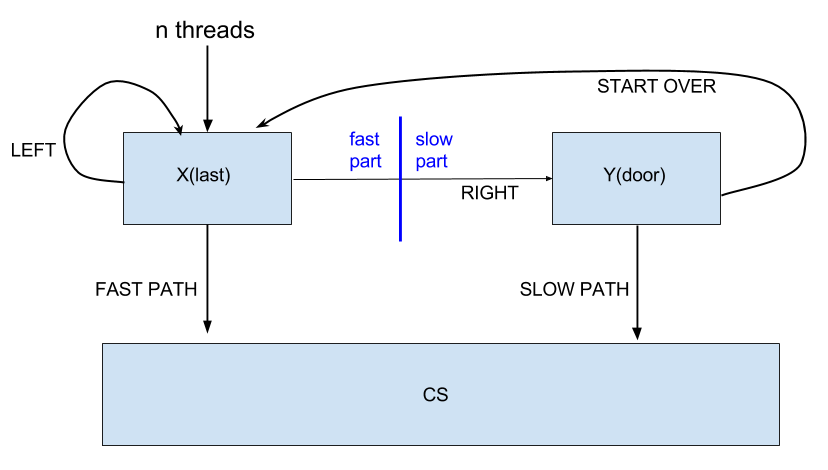
\includegraphics[width=0.72\textwidth]{1.png}
  \caption{Fast Mutex Algorithm Model}
    \label{model}
\end{figure}

Explanation for this algorithm:

There are two shared registers, $X$ and $Y$, that each processor and read and write. For $X$, it holds the last process that acquires permission to get into the critical session and is initially set to -1. For $Y$, it simulates the door, $Y = -1$ indicates the door is open and $Y = i$ means door closed and process $P_i$ is the last one that get entered the door. Also, there are n-length array $flag[n]$ for each process, $flag[i]$ could be $up$ or $down$, $up$ means $P_i$ is contending for mutex using the fast path, $down$ means other cases.

As can see from Figure \ref{model}, at first, process $P_i$ goes into block $X$, set $X = i$, $flag[i] = up$ and check if the door is open($Y=-1$). If not open($Y>=0$), it would go to the \textbf{left} route and try acquiring again some later. If open($Y=-1$), it would close the door by setting $Y = i$ and check if the last acquiring process is still itself ($X=i$), if so, it would go into CS through the \textbf{fast} route, if not, go to the $Y$ block through the \textbf{right} route and set $flag[i] = down$. The last chance to get into CS in this iteration is to wait all flags to be down(which means that no process is in the CS) and if so, at this moment, if the last door-closing process is still $P_i$, then it will enter CS through the \textbf{slow} route, otherwise it would start over and try acquiring again.

To sum, Lamport’s Fast Mutex Algorithm can guarantee deadlock-free but can not guarantee starvation-free. Fast Mutex Algorithm improves Splitter method that it expands Splitter model as two part, fast part and slow part. For fast part, the \textbf{down} route in fast part is similar as the \textbf{down} route in Splitter, can guarantee that the \textbf{\textbar Down\textbar }, the number of threads through down route, is no more than 1, but could be 0. When this case happens, there is nothing in CS, so the slow part could help this algorithm to pick one thread enter CS through slow path, to ensure there is no deadlock. But unlike PetersonN Algorithm, Fast Mutex Algorithm is not first-come-first-serve algorithm, which means the first-come thread might have to wait infinitely. Thus it cannot guarantee starvation-free.

\section{Basic synchronized constructs of OpenMP}

OpenMP(Open Multi-Processing)\cite{1} is an application programming interface (API) that supports multi-platform shared memory multiprocessing programming in C, C++, and Fortran. By using openMP, it is easier to convert a serial code into parallel and also can run the same code as serial code. Figure \ref{openmp} shows that openMP can run parallel code as serial flow, it can control when to distribute main thread into parallel processes and when to merge all parts as a real sequential program.

\begin{figure}[!ht]
  \centering
    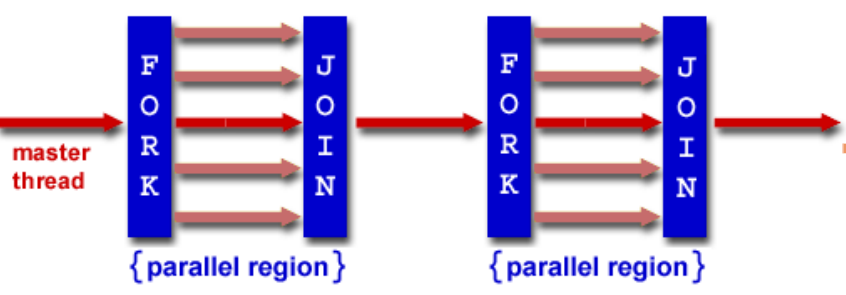
\includegraphics[width=0.72\textwidth]{2.png}
  \caption{Simple Fork-Join Parallelism\cite{2}}
    \label{openmp}
\end{figure}

Most of the constructs in OpenMP are compiler directives. For example:\\
\centerline{$\# pragma\ omp\ parallel\ num\_threads(4)$}\\
is to set the number of threads as 4 (there is always one master thread as the main thread so to create 4 threads means to create 3 more threads besides the master thread).

\subsection{OpenMP variables}

Now we will introduce several variables of OpenMP with examples and explanation\cite{3}.

\subsubsection{Critical}
\begin{table}[!ht]
    \centering
    \begin{tabular}{l  l  l }
    \hline
        \rownumber & float result;  \\ 
        \rownumber & {\color{red}$\#$pragma omp parallel} \\ 
        \rownumber & \{ \\ 
        \rownumber & \ \ \ \ float B; int i, id, nthrds; \\ 
        \rownumber & \ \ \ \ id = omp\_get\_thread\_num();  \\ 
        \rownumber & \ \ \ \ nthrds = omp\_get\_num\_threads(); \\ 
        \rownumber & \ \ \ \ for(i=id; i $<$ N; i = i+nthrds) \{  \\ 
        \rownumber & \ \ \ \ \ \ \ \ B = foo(i); & // expensive computation \\ 
        \rownumber & \ \ \ \ {\color{red}$\#$pragma omp critical} \\ 
        \rownumber & \ \ \ \ \ \ \ \ consume(B, result); \\ 
        \rownumber & \ \ \ \ \} \\
        \rownumber & \} \\
        \hline
    \end{tabular}
    \caption*{Variable Critical}
\end{table}
\setcounter{magicrownumbers}{0}
Variable $critical$ indicates Critical Session, in the code, we have n processors and can execute all iterations in the for-loop at the same time but only one thread would run $Line 10$ at a time.

\subsubsection{Atomic}
\begin{table}[!ht]
    \centering
    \begin{tabular}{l  l  l }
    \hline
        \rownumber & int  n,r;  \\ 
        \rownumber & {\color{red}$\#$pragma omp parallel shared(n,r)} \\ 
        \rownumber & \{ \\ 
        \rownumber & \ \ \ \ for(i=0; i $<$ n; i++) \{  \\ 
        \rownumber & \ \ \ \ {\color{red}$\#$pragma omp atomic} \\ 
        \rownumber & \ \ \ \ \ \ \ \ r += foo(i); & // expensive computation \\ 
        \rownumber & \ \ \ \ \} \\
        \rownumber & \} \\
        \hline
    \end{tabular}
    \caption*{Variable Atomic}
\end{table}
\setcounter{magicrownumbers}{0}
Variable $atomic$ specifies that a memory location that will be updated atomically. For the code, all $foo(i)$ can be executed by n threads at the same time, but $r$ will be updated atomically. 

\subsubsection{Reduction}
\begin{table}[!ht]
    \centering
    \begin{tabular}{l  l  l }
    \hline
        \rownumber & double sum=0.0, ave, A[MAX]; int i;  \\ 
        \rownumber & {\color{red}$\#$pragma omp parallel for reduction (+ $\colon$ sum)} \\ 
        \rownumber & for(i=0; i $<$ MAX; i++) \{  \\ 
        \rownumber & \ \ \ \ sum += A[i];  \\ 
        \rownumber & \} \\
        \rownumber & ave = sum/MAX;\\
        \hline
    \end{tabular}
    \caption*{Variable Reduction}
\end{table}
\setcounter{magicrownumbers}{0}
Variable $reduction$ specifies that one or more variables that are private to each thread are the subject of a reduction operation at the end of the parallel region. For the above code, local copies of variable $sum$ would be created and then combined.

\subsubsection{Barrier}

Variable $barrier$ synchronizes all threads in a team; all threads pause at the barrier, until all threads execute the barrier.

\subsubsection{Master construct}

The target region will be executed only by the $master$ thread.

\subsubsection{Single construct}
\begin{table}[!ht]
    \centering
    \begin{tabular}{l  l  l }
    \hline
        \rownumber & {\color{red}$\#$pragma omp parallel} \\ 
        \rownumber & \{ \\ 
        \rownumber & \ \ \ \ do\_many\_things();  \\ 
        \rownumber & \ \ \ \ {\color{red}$\#$pragma omp single} \\ 
        \rownumber & \ \ \ \ \{exchange\_boundaries();\} & // target region \\ 
        \rownumber & \ \ \ \ {\color{red}$\#$pragma omp barrier } \\ 
        \rownumber & \ \ \ \ do\_many\_other\_things();  \\ 
        \rownumber & \} \\
        \hline
    \end{tabular}
    \caption*{Variable Single construct}
\end{table}
\setcounter{magicrownumbers}{0}
The target region will be executed by just one thread (any thread, not necessary the master). In this case, $Line\ 5$ would be executed by one thread, if the construct here is $master$ instead of $single$, $Line\ 5$ would only be executed by master thread. And after $Line\ 5$, there is a barrier at $Line\ 6$, which makes other threads waiting for the working threads finish their work and then go to $Line\ 7$ at the same time.

\subsubsection{Ordered}

Locations updated in any order but printed in sequential order.

\subsubsection{Lock}

\forceindent $\bullet$ omp\_init\_lock() -- Initializes a simple lock.\\
\forceindent $\bullet$ omp\_set\_lock() -- Blocks thread execution until a lock is available.\\
\forceindent $\bullet$ omp\_unset\_lock()  -- Releases a lock.\\
\forceindent $\bullet$ omp\_test\_lock()  -- Attempts to set a lock but does not block thread execution.\\
\forceindent $\bullet$ omp\_destroy\_lock() -- Uninitializes a lock.

\subsection{OpenMP data attributes}

\forceindent $\bullet$ $Shared$ variable is shared among threads.\\
\forceindent $\bullet$ $Private$ variable($var$) creates a new local copy of $var$ for each thread.\\
\forceindent $\bullet$ $Firstprivate$ variable initializes each private copy with the corresponding value from the \textbf{master} thread.\\
\forceindent $\bullet$ $Lastprivate$ variable passes the value of a private from the \textbf{last} iteration to a global variable.



\begin{table}[!ht]
    \centering
    \begin{tabular}{l  l  l }
    \hline
        \rownumber & void Foo() \\ 
        \rownumber & \{ \\ 
        \rownumber & \ \ \ \ int tmp = 0;  \\ 
        \rownumber & \ \ \ \ {\color{red}$\#$pragma omp for private(tmp)}/ \\
        \rownumber & \ \ \ \ {\color{red}$\#$pragma omp for firstprivate(tmp)}/ \\ 
        \rownumber & \ \ \ \ {\color{red}$\#$pragma omp for firstprivate(tmp) lastprivate(tmp)} \\ 
        \rownumber & \ \ \ \ \ \ \ \ for(int j = 0;j $<$ 100; j++ ) \{ \\ 
        \rownumber & \ \ \ \ \ \ \ \ tmp += j; \\ 
        \rownumber & \ \ \ \ \ \ \ \ printf(``\%d\textbackslash n'', tmp);  \\ 
        \rownumber & \ \ \ \ \} \\
        \rownumber & \} \\
        \hline
    \end{tabular}
    \caption*{OpenMP data attributes}
\end{table}
\setcounter{magicrownumbers}{0}

See the example on next page. We can pick one line from those three: $Line\ 4$, $Line\ 5$, $Line\ 6$. $Line\ 4$ indicates that the value($tmp$) is uninitialized and undefined after the region. $Line\ 5$ indicates that all copies have value of $tmp$ initialized as 0. $Line\ 6$ indicates that not only all copies have value of $tmp$ initialized as 0, but after the $for$ loop, the variable $tmp$ has the value from the last iteration (i.e. j=99). 

\subsection{Dijkstra Algorithm}
Dijkstra code example with OpenMP implementation can be seen from \cite{4}.

\section{Solve the puzzle}

From previous lectures, we have three ways to solve the find-maximum-from-N-numbers puzzle, listed as Table \ref{table:1}
\begin{table}[H]
    \centering
    \begin{tabular}{ |c||c|c| } 
        \hline
        Algorithm & Work & Time \\
        \hline
        \hline
        Sequential & O($N$) & O($N$) \\ 
        \hline
        Binary & O($N$) & O($log(N)$) \\ 
        \hline
        All-pair Algorithm & O($N^2$) & O($1$) \\   
        \hline
    \end{tabular}
    \caption{Previous result of solving the puzzle}
    \label{table:1}
\end{table}

Now we will discuss two new methods to solve the puzzle with better performance.

\subsection{DoublyLog Algorithm}

In All-pair Algorithm, we have the idea that we can divide the N numbers into $\sqrt{N}$ groups with each group has $\sqrt{N}$ numbers. To expand that, we can more deeply divide each $\sqrt{N}$ groups into $\sqrt{\sqrt{N}}$ sub-groups and keep dividing until the size of each group is only 1 or 2. This idea is shown in Figure \ref{doublylog}.

\begin{figure}[!ht]
  \centering
    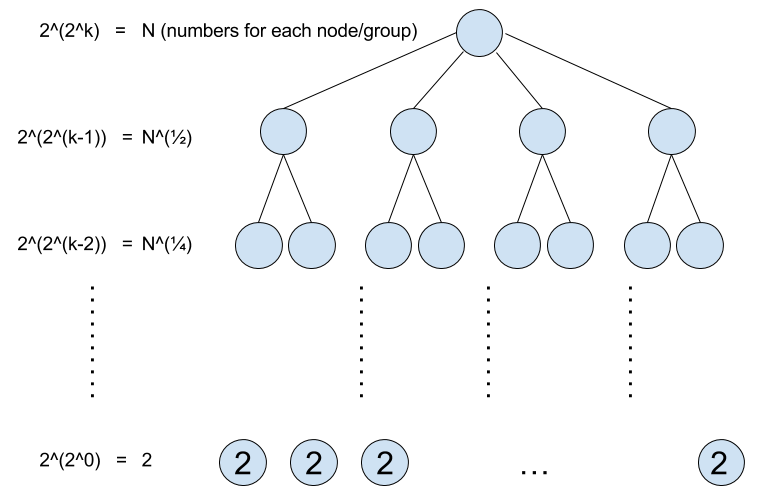
\includegraphics[width=0.7\textwidth]{3.png}
  \caption{DoublyLog Algorithm Model}
    \label{doublylog}
\end{figure}

The height of this tree is $k$, which is $log(log(N))$, if we have enough processors, the time complexity will be the number of layers, which is $O(log(log(N)))$, and for each layer, the work we will be $O(N)$, so the total work will be $O(Nlog(log(N)))$.

\subsection{Cascaded Algorithm}

To better improve the performance, we try to cascade two different methods to get benefit from both of them. In Cascaded Algorithm, we synthesize Sequential Algorithm and DoublyLog Algorithm.

We divide $N$ numbers into $log(log(N))$-length groups, which means there are $N/log(log(N))$ groups. With sequential algorithm, we can get $N/log(log(N))$ maximum candidates, and then we get the final maximum by compare these candidates using DoublyLog Algorithm. This idea is shown in Figure \ref{cascaded}.

\begin{figure}[!ht]
  \centering
    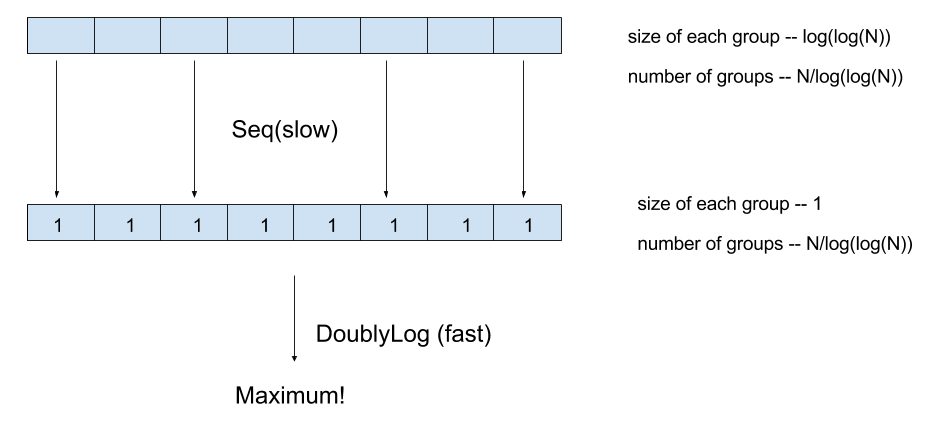
\includegraphics[width=0.85\textwidth]{4.png}
  \caption{Cascaded Algorithm Model}
    \label{cascaded}
\end{figure}


For the first part, work complexity for sequential is $O(N)$ and time complexity is size of each group, which is $O(log(log(N)))$. For the second part, according to DoublyLog ALgorithm, work complexity is $N/(log(log(N)))*(log(log(N)))=O(N)$, and time complexity is still $O(log(log(N)))$.
Now we can expand Table \ref{table:1} as Table \ref{table:2}.
\begin{table}[H]
    \centering
    \begin{tabular}{ |c||c|c| } 
        \hline
        Algorithm & Work & Time \\
        \hline
        \hline
        Sequential & O($N$) & O($N$) \\ 
        \hline
        Binary & O($N$) & O($log(N)$) \\ 
        \hline
        All-pair Algorithm & O($N^2$) & O($1$) \\   
        \hline
        \hline
        DoublyLog Algorithm & O($N*log(log(N))$) & O($log(log(N))$) \\   
        \hline
        Cascaded Algorithm & O($N$) & O($log(log(N))$) \\   
        \hline
    \end{tabular}
    \caption{Current result of solving the puzzle}
    \label{table:2}
\end{table}

\subsection{New puzzle}
We have two sorted arrays, say $A[m]$ and $B[n]$, how could we merge them into a larger array, say $C[m+n]$, in parallel?

\section*{References}
\beginrefs
%\bibentry{1}{\sc V.K.~Garg} Introduction to Multicore Computing
\bibentry{1} https://en.wikipedia.org/wiki/OpenMP
\bibentry{2} http://www.llnl.gov/computing/tutorials/openMP
\bibentry{3} https://msdn.microsoft.com
\bibentry{4} https://github.com/vijaygarg1/UT-Garg-EE382C-EE361C-Multicore/blob/master/openMP/Dijkstra.c
\endrefs


\end{document}





